\documentclass{article}

% import packages
\usepackage{amsmath,amsfonts,amsthm,amssymb,amsopn,bm}
\usepackage{mathtools}
\usepackage[margin=.9in]{geometry}
\usepackage{graphicx}
\usepackage[dvipsnames]{xcolor}
\usepackage{minted}
\usepackage{subcaption}
\usepackage{float}

% note command
\newcommand{\note}[1]{\textsf{\textcolor{Red}{#1}}}

% some math commands
\newcommand{\norm}[1]{\left\|#1\right\|}
\newcommand{\twonorm}[1]{\|#1\|_2^2}
\newcommand{\vect}[1]{\boldsymbol{#1}} % vector 
\DeclareMathOperator{\E}{\mathbb{E}}
\DeclareMathOperator{\cov}{Cov}
\DeclareMathOperator{\var}{Var}

% remove indents
\setlength\parindent{0px}
% enumerate with lowercase letters
\renewcommand{\theenumi}{\alph{enumi}}
% indented environment for solutions
\usepackage{changepage}
\newenvironment{solution}{\begin{adjustwidth}{8mm}{}}{\end{adjustwidth}}

% macro for Gaussian elimination
\usepackage{array}
\makeatletter
\newcounter{elimination@steps}
\newcolumntype{R}[1]{>{\raggedleft\arraybackslash$}p{#1}<{$}}
\def\elimination@num@rights{}
\def\elimination@num@variables{}
\def\elimination@col@width{}
\newenvironment{elimination}[4][0]
{
    \setcounter{elimination@steps}{0}
    \def\elimination@num@rights{#1}
    \def\elimination@num@variables{#2}
    \def\elimination@col@width{#3}
    \renewcommand{\arraystretch}{#4}
    \start@align\@ne\st@rredtrue\m@ne
}
{
    \endalign
    \ignorespacesafterend
}
\newcommand{\eliminationstep}[2]
{
    \ifnum\value{elimination@steps}>0\hspace{-1.2cm}\to\quad\fi
    \left[
        \ifnum\elimination@num@rights>0
            \begin{array}
            {@{}*{\elimination@num@variables}{R{\elimination@col@width}}
            |@{}*{\elimination@num@rights}{R{\elimination@col@width}}}
        \else
            \begin{array}
            {@{}*{\elimination@num@variables}{R{\elimination@col@width}}}
        \fi
            #1
        \end{array}
    \right]
    & 
    \begin{array}{l}
        #2
    \end{array}
    &%                                    moved second & here
    \addtocounter{elimination@steps}{1}
}
\makeatother


% Homework title and date
\renewcommand{\title}{Homework 0 A}
\renewcommand{\date}{October 5, 2020}

\begin{document}

\begin{center}
        \LARGE \title \\ \vspace{10pt}
        \normalsize 
        Fall 2020, CSE 546: Machine Learning \\ \vspace{2pt}
        John Franklin Crenshaw \\ \vspace{2pt}
        \date
\end{center}

%Collaborators:

\section*{Probability and Statistics}

\textbf{A.1} 
(Bayes Rule, from Murphy exercise 2.4) 
After your yearly checkup, the doctor has bad news and good news. 
The bad news is that you tested positive for a serious disease, and that the test is 99\% accurate (i.e., the probability of testing positive given that you have the disease is 0.99, as is the probability of testing negative given that you don't have the disease).
The good news is that this is a rare disease, striking only one in 10,000 people. 
What are the chances that you actually have the disease?
(Show your calculations as well as giving the final result) \newline

\begin{solution}
        Let $A$ denote having the disease, and $B$ denote testing positive for the disease.
        We are given $p(B|A) = 0.99$, $p(A) = 10^{-4}$.
        Using these, we can calculate 
        \begin{align*}
                p(B) = p(B|A)p(A) + p(B|\neg A)p(\neg A) = 0.99 \cdot 10^{-4} + (1-0.99) \cdot (1-10^{-4}) \approx 0.01
        \end{align*}
        Finally, using Bayes' Theorem, we have.
        \begin{align*}
                p(A|B) = p(B|A) ~ \frac{p(A)}{p(B)} = 0.99 \cdot \frac{10^{-4}}{0.01} \approx 0.01
        \end{align*}
        So there's only a 1\% chance you actually have the disease.
\end{solution} \vspace{10pt}


\textbf{A.2}
For any two random variables $X,Y$ the \textit{covariance} is defined as $\cov(X,Y) = \E[(X - \E[x])(Y- \E[Y])]$.

\begin{enumerate}
        \item If $\E[Y|X=x]=x$ show that $\cov(X,Y) = \E[(X-\E[X])^2]$.
        \begin{solution}
                \vspace{-5mm}
                \begin{align*}
                        \cov(X,Y) 
                        &= \E[(X - \E[X])(Y- \E[Y])] \\
                        &= \E[XY - X\E[Y] - \E[X]Y + \E[X]\E[Y]] \\
                        &= \E[XY] - \E[X]\E[Y] - \E[X]\E[Y] + \E[X]\E[Y] \\
                        &= \E[XY] - \E[X]\E[Y] \\
                        \E[XY]
                        &= \int x y \, p(x,y) \, dx \, dy
                         = \int x y \, p(y|x) \, p(x) \, dx \, dy \\
                        &= \int x \, p(x) \left[ \int y \, p(y|x) \, dy \right] dx
                         = \int x^2 \, p(x) dx = \E[X^2] \\
                        \E[Y]
                        &= \int y \, p(y) \, dy 
                         = \int y \, p(y|x) \, p(x) \, dy \, dx \\
                        &= \int p(x) \left[ \int y \, p(y|x) \, dy \right] dx 
                         = \int x \, p(x) \, dx = \E[X]
                \end{align*}
                where I substituted $\E[Y|X=x]=x$ for the integrals in brackets above.
                Finally,
                \begin{align*}
                        \E[(X - \E[X])^2] 
                        &= \E[X^2 - 2X\E[X] + \E[X]^2] \\
                        &= \E[X^2] - 2\E[X]^2 + \E[X]^2 \\
                        &= \E[X^2] - \E[X]^2 \\
                        &= \cov(X,Y),
                \end{align*}
                which proves the desired result.
        \end{solution}
        \item If $X,Y$ are independent, show that $\cov(X,Y) = 0$.
        \begin{solution}
                Above I showed $\cov(X,Y) = \E[XY] - \E[X]\E[Y]$. 
                If $X,Y$ are independent, then $\E[XY] = \E[X]\E[Y]$, as the integrals factor.
                Thus $\cov(X,Y) = \E[X]\E[Y] - \E[X]\E[Y] = 0$
        \end{solution}
\end{enumerate}


\textbf{A.3}
Let $X$ and $Y$ be independent random variables with PDFs given by $f$ and $g$, respectively. 
Let $h$ be the PDF of the random variable $Z = X + Y$.

\begin{enumerate}
        \item Show that $h(z) = \int_{-\infty}^{\infty} f(x) g(z-x) dx$
        \begin{solution}
                We can write $h(z)$ as an integral over values of $x$:
                \begin{align*}
                        h(z) = \int_{-\infty}^{\infty} p(z|x) f(x) dx.
                \end{align*}
                Now as $Z = X + Y$, the conditional probability $p(z|x)$ is the same as asking what's the probability that $y = z - x$, i.e. $p(z|x) = g(z-x)$.
                Putting it all together,
                \begin{align*}
                        h(z) = \int_{-\infty}^{\infty} f(x) g(z-x) dx.
                \end{align*}
        \end{solution}
        \item If $X$ and $Y$ are both independent and uniformly distributed on $[0,1]$ (i.e. $f(x) = g(x) = 1$ for $x \in [0,1]$ and 0 otherwise), what is $h$, the PDF of $Z = X + Y$?
        \begin{solution}
                Clearly $h(z) = 0$ when $z<0$ or $z>2$, as you are adding two random numbers between 0 and 1.
                Now for $g(z-x) \neq 0$, we must have $z-1 \leq x \leq z$.
                Combining these limits with the limits $0 \leq x \leq 1$, we have two different cases:
                \begin{align*}
                        z < 1 &: \quad h(z|z<1) = \int_0^z dz = z \\
                        z \geq 1 &: \quad h(z|z \geq 1) = \int_{z-1}^1 dz = 2 - z 
                \end{align*}
        So the PDF for $z$ is 
        \begin{align*}
                h(z) = 
                \begin{cases}
                        z & 0 < z \leq 1 \\
                        2-z & 1 < z < 2 \\
                        0 &\text{otherwise}        
                \end{cases}
        \end{align*}
        \end{solution}
\end{enumerate}


\textbf{A.4}
A random variable $X \sim \mathcal{N}(\mu,\sigma^2)$ is Gaussian distributed with mean $\mu$ and variance $\sigma^2$.
Given that for any $a,b \in \mathbb{R}$, we have that $Y = aX + b$ is also Gaussian, find $a,b$ such that $Y \sim \mathcal{N}(0,1)$.

\begin{solution}
        \vspace{-5mm}
        \begin{align*}
                \E[Y] &= \E[aX + b] = a\E[X] + b = a\mu + b = 0 \\
                \var[Y] &= \var[aX+b] = a^2 \var[X] = a^2 \sigma^2 = 1 \\
                \Rightarrow& \quad a = \sigma^{-1}, \quad b = \frac{\mu}{\sigma}
        \end{align*}
\end{solution}


\textbf{A.5}
For a random variable $Z$, its mean and variance are defined as $\E[Z]$ and $\E[(Z-\E[Z])^2]$, respectively.
Let $X_1, \dots, X_n$ be independent and identically distributed random variables, each with mean $\mu$ and variance $\sigma^2$.
If we define $\hat{\mu}_n = \frac{1}{n} \sum_{i=1}^n X_i$, what is the mean and variance of $\sqrt{n}(\hat{\mu}_n - \mu)$? \newline

\begin{solution}
        \vspace{-5mm}
        \begin{align*}
                \E \left[ \sqrt{n}(\hat{\mu}_n - \mu) \right] 
                &= \sqrt{n} \left( \E[\hat{\mu}_n] - \mu \right) 
                 = \sqrt{n} \left( \frac{1}{n} \sum_{i=1}^n \E[X_i] - \mu \right) \\
                &= \sqrt{n} \left( \frac{1}{n} \sum_{i=1}^n \mu - \mu \right) 
                 = \sqrt{n} (\mu - \mu) = 0 \\
                \var \left[ \sqrt{n}(\hat{\mu}_n - \mu) \right]
                &= \var \left[ \sqrt{n} \hat{\mu}_n \right] = n \var \left[ \frac{1}{n} \sum_{i=1}^n X_i \right] = \frac{1}{n} \sum_{i,j = 1}^n \cov(X_i,X_j) \\
                &= \frac{1}{n} \sum_{i = 1}^n \var(X_i) = \frac{1}{n} \cdot n \sigma^2 = \sigma^2
        \end{align*}
        In the last line I used the fact that the $X_i$ are uncorrelated (i.e. $\cov(X_i,X_j) = 0, ~ \forall i \neq j$).
\end{solution}


\textbf{A.6}
If $f(x)$ is a PDF, the cumulative distribution function (CDF) is defined as $F(X)=\int_{-\infty}^x f(y)dy$.
For any function $g ~:~ \mathbb{R} \to \mathbb{R}$ and random variable $X$ with PDF $f(x)$, recall that the expected value of $g(x)$ is defined as $\E[g(X)] = \int_{-\infty}^{\infty} g(y)f(y) dy$.
For a boolean event $A$, define $\vect{1}\{A\}$ as 1 if $A$ is true, and 0 otherwise.
Thus, $\vect{1}\{x \leq a\}$ is 1 whenever $x \leq a$ and 0 whenever $x > a$.
Note that $F(x) = \E[\vect{1}\{X \leq x\}]$.
Let $X_1, \dots, X_n$ be \textit{independent and identically distributed} random variables with CDF $F(x)$.
Define $\hat{F}_n(x) = \frac{1}{n} \sum_{i=1}^n \vect{1}\{X_i \leq x\}$.
Note, for every $x$, that $\hat{F}_n(x)$ is an \textit{empirical estimate} of $F(x)$.
You may use your answers to the previous problem.

\begin{enumerate}
        \item For any $x$, what is $\E[\hat{F}_n(x)]$?
        \begin{solution}
                \vspace{-5mm}
                \begin{align*}
                        \E[\hat{F}_n(x)] 
                        = \E[\frac{1}{n} \sum_{i=1}^n \vect{1}\{X_i \leq x\}]
                        = \frac{1}{n} \sum_{i=1}^n \E[\vect{1}\{X_i \leq x\}]
                        = \frac{1}{n} \sum_{i=1}^n F(x)
                        = \frac{1}{n} \cdot n \, F(x)
                        = F(x)                        
                \end{align*}
        \end{solution}
        \item For any $x$, the variance of $\hat{F}_n(x)$ is $\E[(\hat{F}_n(x) - F(x))^2]$.
                Show that $\var(\hat{F}_n(x)) = \frac{F(x)(1-F(x))}{n}$.
        \begin{solution}
                \note{NEED TO FINISH THIS PROBLEM}
        \end{solution}
\end{enumerate}


\section*{Linear Algebra and Vector Calculus}

\textbf{A.7}
(Rank)
Let $A = \begin{bmatrix} 
                1 & 2 & 1 \\
                1 & 0 & 3 \\ 
                1 & 1 & 2 
        \end{bmatrix}$ 
        and 
        $B = \begin{bmatrix} 
                1 & 2 & 3 \\ 
                1 & 0 & 1 \\ 
                1 & 1 & 2 
        \end{bmatrix}$.
For each matrix $A$ and $B$,

\begin{enumerate}
        \item what is its rank?
        \begin{solution}
                The characteristic polynomial of $A$ is 
                $\det(A - \lambda I) = -\lambda^3 + 3\lambda^2 + 4\lambda = -\lambda(\lambda - 4) (\lambda + 1)$.
                As the characteristic polynomial has three distinct roots, $A$ is diagonalizable.
                Since two of the roots are non-zero, $\text{rank} (A) = 2$.

                The characteristic polynomial of $B$ is
                $\det(B - \lambda I) = -\lambda^3 + 3\lambda^2 + 4\lambda$, which is the same as $A$.
                Therefore, $\text{rank} (B) = \text{rank} (A) = 2$
        \end{solution}
        \item what is a (minimal size) basis for its column span?
        \begin{solution}
                The dimension of the column space of a matrix is equal to its rank.
                Thus for each matrix, we need two basis vectors.
                We can see that the first two columns of both matrices are linearly independent of one another (and are the same for both matrices).
                So a basis for the column span of both matrices is 
                \begin{align*}
                        \left\{
                        \begin{bmatrix} 1 \\ 1 \\ 1 \end{bmatrix},
                        \begin{bmatrix} 2 \\ 0 \\ 1 \end{bmatrix}
                        \right\}
                \end{align*}
        \end{solution}
\end{enumerate}


\textbf{A.8}
(Linear equations)
Let $A = \begin{bmatrix} 
                0 & 2 & 4 \\ 
                2 & 4 & 2 \\ 
                3 & 3 & 1 
        \end{bmatrix}$, 
        $b = \begin{bmatrix} 
                -2 & -2 & -4 
        \end{bmatrix}^T$, 
        and $c=\begin{bmatrix} 
                1 & 1 & 1 
        \end{bmatrix}^T$.

\begin{enumerate}
        \item What is $Ac$?
        \begin{solution}
                \vspace{-5mm}
                \begin{align*}
                        Ac = 
                        \begin{bmatrix}
                                0 \cdot 1 + 2 \cdot 1 + 4 \cdot 1 \\
                                2 \cdot 1 + 4 \cdot 1 + 2 \cdot 1 \\
                                3 \cdot 1 + 3 \cdot 1 + 1 \cdot 1 
                        \end{bmatrix} 
                        = \begin{bmatrix} 6 \\ 8 \\ 7 \end{bmatrix}
                \end{align*}
        \end{solution}
        \item What is the solution to the linear system $Ax=b$?
        \begin{solution}
                Using Gaussian elimination:
                \begin{elimination}[1]{3}{1.5em}{1.1}
                        \eliminationstep
                        {
                                0 & 2 & 4 & -2 \\
                                2 & 4 & 2 & -2 \\
                                3 & 3 & 1 & -4
                        }
                        {
                                \cdot ~ \frac{1}{2}\\
                                -2 R_1 \\
                                -\frac{3}{2} R_1
                        }
                        \eliminationstep
                        {
                                0 & 1 &  2 & -1 \\
                                2 & 0 & -6 &  2 \\
                                3 & 0 & -5 & -1
                        }
                        {
                                \\
                                \cdot ~ \frac{1}{2} \\
                                -\frac{3}{2} R_2 \\
                        } \\
                        \eliminationstep
                        {
                                0 & 1 &  2 & -1 \\
                                1 & 0 & -3 &  1 \\
                                0 & 0 &  4 & -4
                        }
                        {
                                - \frac{1}{2} R_3\\
                                + \frac{3}{4} R_3 \\
                                \cdot ~ \frac{1}{4} \\
                        }
                        \eliminationstep
                        {
                                0 & 1 & 0 &  1 \\
                                1 & 0 & 0 & -2 \\
                                0 & 0 & 1 & -1
                        }{}
                \end{elimination}
                So $x = \begin{bmatrix} -2 & 1 & -1 \end{bmatrix}^T$.
        \end{solution}
\end{enumerate}


\textbf{A.9}
(Hyperplanes)
Assume $w$ is an $n$-dimensional vector and $b$ is a scalar.
A hyperplane in $\mathbb{R}^n$ is the set $\{ x : x \in \mathbb{R}^n, ~ \text{s.t.} ~ w^T x + b = 0 \}$.

\begin{enumerate}
        \item ($n = 2$ example)
                Draw the hyperplane for $w = \begin{bmatrix} -1 & 2 \end{bmatrix}^T$, $b=2$.
        \begin{solution}
                This is the equation $-x_1 + 2x_2 + 2 = 0$, or $x_2 = \frac{1}{2} x_1 - 1$.
                \begin{figure}[h]
                        \begin{subfigure}{0.5\linewidth}
                                \centering
                                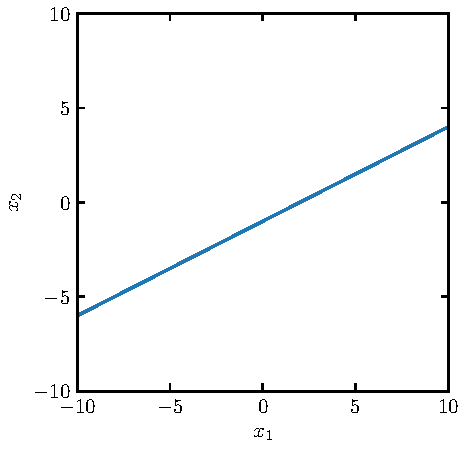
\includegraphics[width=\linewidth]{A9a.pdf}
                        \end{subfigure}
                        \hfill
                        \begin{subfigure}{0.40\linewidth}
                                \centering
                                \begin{minted}[autogobble]{python}
                                        import numpy as np
                                        import matplotlib.pyplot as plt
                        
                                        x1 = np.linspace(-10,10)
                                        x2 = 1/2 * x1 - 1
                        
                                        plt.plot(x1,x2)
                                        plt.xlabel('$x_1$')
                                        plt.ylabel('$x_2$')
                                \end{minted}
                        \end{subfigure}
                \end{figure}
        \end{solution}
        \item ($n = 3$ example)
                Draw the hyperplane for $w = \begin{bmatrix} 1 & 1 & 1 \end{bmatrix}^T$, $b=0$.
        \begin{solution}
                This is the equation $x_1 + x_2 + x_3 = 0$, or $x_3 = -x_1 - x_2$.
                \begin{figure}[h]
                        \begin{subfigure}{0.5\linewidth}
                                \centering
                                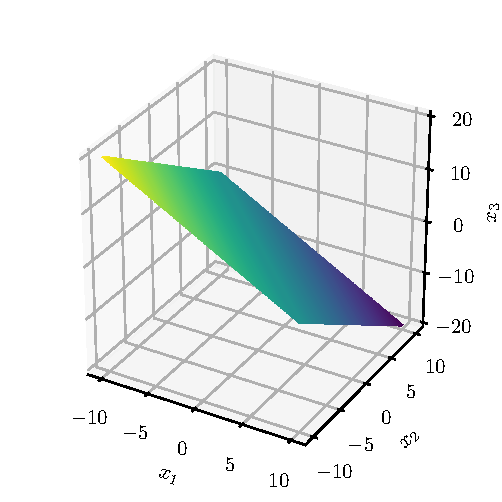
\includegraphics[width=\linewidth]{A9b.pdf}
                        \end{subfigure}
                        \hfill
                        \begin{subfigure}{0.40\linewidth}
                                \centering
                                \begin{minted}[autogobble]{python}
                                        import numpy as np
                                        import matplotlib.pyplot as plt
                                        from mpl_toolkits import mplot3d

                                        x1 = np.linspace(-10,10)
                                        x2 = np.linspace(-10,10)
                                        x1grid, x2grid = np.meshgrid(x1,x2)
                                        x3grid = -x1grid - x2grid

                                        fig = plt.figure(constrained_layout=True)
                                        ax = plt.axes(projection='3d')

                                        ax.contour3D(x1grid, x2grid, x3grid, 300)
                                        ax.set_xlabel("$x_1$")
                                        ax.set_ylabel("$x_2$")
                                        ax.set_zlabel("$x_3$")
                                        ax.dist=11
                                \end{minted}
                        \end{subfigure}  
                \end{figure}
        \end{solution}
        \item Given some $x_0 \in \mathbb{R}^n$, find the \textit{squared distance} to the hyperplane defined by $w^Tx+b=0$.
        In other words, solve the following optimization problem:
        \begin{align*}
                \min_x \norm{x_0 - x}^2 \\
                \text{s.t. } w^Tx+b = 0
        \end{align*}
        \begin{solution}
                As $w$ is normal to the plane, $w$ and $(x_0 - \tilde{x}_0)$ are parallel or anti-parallel.
                Thus, 
                \begin{align*}
                        |w^T (x_0 - \tilde{x}_0)| = \norm{w} \norm{x_0 - \tilde{x}_0}.
                \end{align*}
                Using the constraint above, $w^T \tilde{x}_0 = -b$.
                Plugging in and rearranging,
                \begin{align*}
                        \norm{x_0 - \tilde{x}_0}^2 = \left( \frac{w^T x_0 + b}{\norm{w}} \right)^2.
                \end{align*}
        \end{solution}
\end{enumerate}


\textbf{A.10}
For possibly non-symmetric $A,B \in \mathbf{R}^{n \times n}$ and $c \in \mathbb{R}$, let $f(x,y) = x^T A x + y^T B x + c$.
Define $\nabla_z f(x,y) = \begin{bmatrix}
        \frac{\partial f(x,y)}{\partial z_1} &
        \frac{\partial f(x,y)}{\partial z_2} &
        \dots &
        \frac{\partial f(x,y)}{\partial z_n}
\end{bmatrix}^T$.

\begin{enumerate}
        \item Explicitly write out the function $f(x,y)$ in terms of the components of $A_{ij}$ and $B_{ij}$ using appropriate summations over the indices.
        \begin{solution}
                \vspace{-5mm}
                \begin{align*}
                        f(x,y) = c + \sum_{i,j} (A_{ij} x_i x_j + B_{ij} y_i x_j)
                \end{align*}
        \end{solution}
        \item What is $\nabla_x f(x,y)$ in terms of the summations over indices \textit{and} vector notation?
        \begin{solution}
                \vspace{-5mm}
                \begin{align*}
                        \text{In index notation:}& \quad 
                        [\nabla_x f(x,y)]_i = \sum_j A_{ij} x_j + A_{ji} x_j + B_{ji} y_j \\
                        \text{In vector notation:}& \quad
                        \nabla_x f(x,y) = (A + A^T) x + B^T y
                \end{align*}
        \end{solution}
        \item What is $\nabla_y f(x,y)$ in terms of the summations over indices \textit{and} vector notation?
        \begin{solution}
                \vspace{-5mm}
                \begin{align*}
                        \text{In index notation:}& \quad 
                        [\nabla_y f(x,y)]_i = \sum_j B_{ij} x_j \\
                        \text{In vector notation:}& \quad
                        \nabla_x f(x,y) = Bx
                \end{align*}
        \end{solution}
\end{enumerate}


\section*{Programming}


\textbf{A.11}
For the $A,b,c$ as defined in Problem 8, use NumPy to compute (take a screenshot of your answer):
\begin{enumerate}
        \item What is $A^{-1}$?
        \begin{solution}
                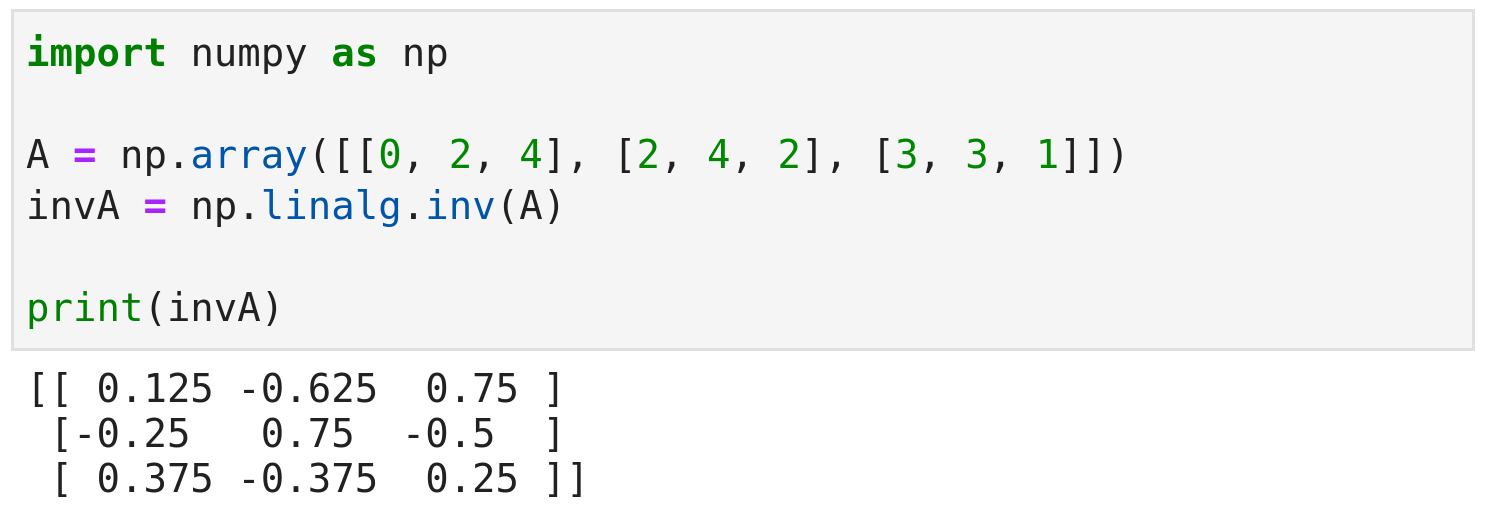
\includegraphics[width=0.7\linewidth]{A11a.png}
        \end{solution}
        \item What is $A^{-1}b$? What is $Ac$?
        \begin{solution}
                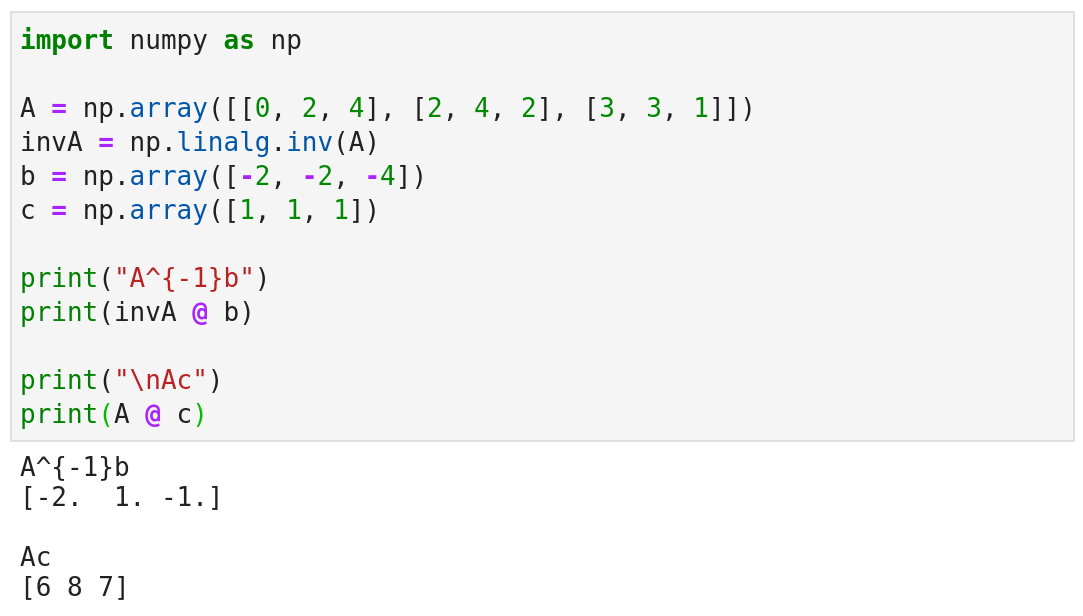
\includegraphics[width=0.72\linewidth]{A11b.png}
        \end{solution}
\end{enumerate}


\textbf{A.12}
Two random variables $X$ and $Y$ have equal distributions if their CDFs, $F_X$ and $F_Y$, respectively, are equal, i.e. for all $x$, $|F_X(x)-F_Y(x)|=0$.
The central limit theorem says that the sum of $k$ independent, zero-mean, variance-$1/k$ variables converges to a (standard) Normal distribution as $k$ goes off to infinity.
We will study this phenomenon empirically (you wil use the Python packages Numpy and Matplotlib).
Define $Y^{(k)} = \frac{1}{\sqrt{k}} \sum_{i=1}^k B_i$ where each $B_i$ is equal to $-1$ and $1$ with equal probability. From your solution to problem A.5, we know that $\frac{1}{\sqrt{k}}B_i$ is zero-mean and has variance $1/k$.

\begin{enumerate}
        \item For $i=1,\dots,n$ let $Z_i \sim \mathcal{N}(0,1)$. If $F(x)$ is the true CDF from which each $Z_i$ is drawn (i.e., Gaussian) and $\hat{F}_n(x) = \frac{1}{n} \sum_{i=1}^n \vect{1}\{Z_i \leq x\}$, use the answer to problem A.6 above to choose $n$ large enough such that, for all $x \in \mathbb{R}$, $\sqrt{\E[(\hat{F}_n(x) - F(x))^2]} \leq 0.0025$, and plot $\hat{F}_n(x)$ from $-3$ to $3$.
        \begin{solution}
                Using the solution for A.6, we have
                \begin{align*}
                        n = \frac{F(x)(1-F(x))}{(0.0025)^2} < \frac{1}{(0.0025)^2} = 1.6 \times 10^5.
                \end{align*}
                See plot and code below.
        \end{solution}
        \item For each $k \in \{1,8,64,512\}$ generate $n$ independent copies $Y^{(k)}$ and plot their empirical CDF on the same plot as part a.
        \begin{solution}
                \begin{figure}[H]
                        \centering
                        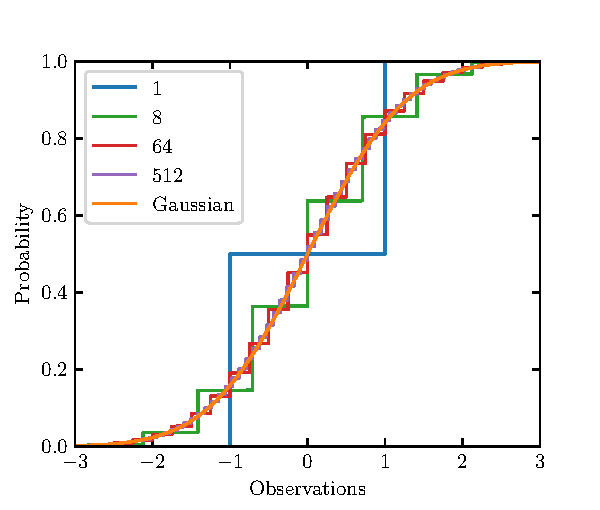
\includegraphics[width=0.5\linewidth]{A12.pdf}
                \end{figure}
                \begin{minted}[autogobble]{python}
                        import numpy as np
                        import matplotlib.pyplot as plt

                        np.random.seed(11)

                        n = int(1.6e5)

                        for k in [1,8,64,512]:
                        Y = np.sum(np.sign(np.random.randn(n, k))*np.sqrt(1/k), axis=1)
                        plt.plot(sorted(Y), np.arange(1,n+1)/float(n), label=k)
                        
                        Z = np.random.randn(n)
                        plt.step(sorted(Z), np.arange(1,n+1)/float(n), label='Gaussian')

                        plt.legend()
                        plt.xlim(-3,3)
                        plt.ylim(0,1)
                        plt.xlabel('Observations')
                        plt.ylabel('Probability')
                \end{minted}
        \end{solution}
\end{enumerate}

\end{document}
